% Toolbar icon: measure — a diagonal ruler between two endpoint dots (distance
% measurement between two picked nodes, inside the Inspect panel).
% NOTE: the committed svg-ui/measure.svg was hand-authored to the same
% drawing (no LaTeX toolchain available); regenerating via `make ui` replaces
% it with the pdftocairo rendering of this source — same glyph either way.
\documentclass[tikz,border=2mm]{standalone}
\usetikzlibrary{arrows.meta,calc}
\begin{document}
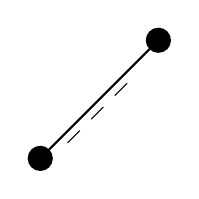
\begin{tikzpicture}[line width=1.3pt, line cap=round, line join=round, x=1mm,y=1mm]
  \draw[thick] (-7.5,-7.5) -- (7.5,7.5);                  % ruler line
  \foreach \t in {-4,-1,2} {
    \draw[thin] (\t,\t-1.5) -- (\t+1.5,\t);                % tick marks
  }
  \fill (-7.5,-7.5) circle (1.6);                          % endpoint dots
  \fill (7.5,7.5) circle (1.6);
\end{tikzpicture}
\end{document}
